\documentclass[12pt]{article}

\usepackage[german,ngerman]{babel}
\usepackage[utf8]{inputenc}
\usepackage[paper=a4paper,left=25mm,right=25mm,top=25mm,bottom=25mm]{geometry}
\usepackage{fancyhdr}
\usepackage{lastpage}
\usepackage{graphicx} 
%\usepackage{multirow}
%\usepackage{draftcopy}
\usepackage{pdfpages}
\usepackage{svg}
\usepackage{array}
\usepackage{draftwatermark}


\SetWatermarkScale{4}
\SetWatermarkText{Entwurf}
\SetWatermarkLightness{0.9}

\pagestyle{fancy}
\fancyhf{} %alle Kopf- und Fußzeilenfelder bereinigen
\fancyhead[L]{Lerne programmieren mit HPL} %zentrierte Kopfzeile
\fancyhead[R]{Didaktische Hinweise} %zentrierte Kopfzeile

\renewcommand{\headrulewidth}{0.4pt} %obere Trennlinie
\fancyfoot[R]{\thepage /\pageref{LastPage}  } %Seitennummer
\fancyfoot[L]{
\includegraphics[width=0.15\textwidth]{Creative_Commons_yy-sa_small} stotz amXa consulting $|$ stotz@amxa.ch }
\renewcommand{\footrulewidth}{0.4pt} %untere Trennlininie

\frenchspacing
\parindent0cm
\parskip0.4em

\begin{document}
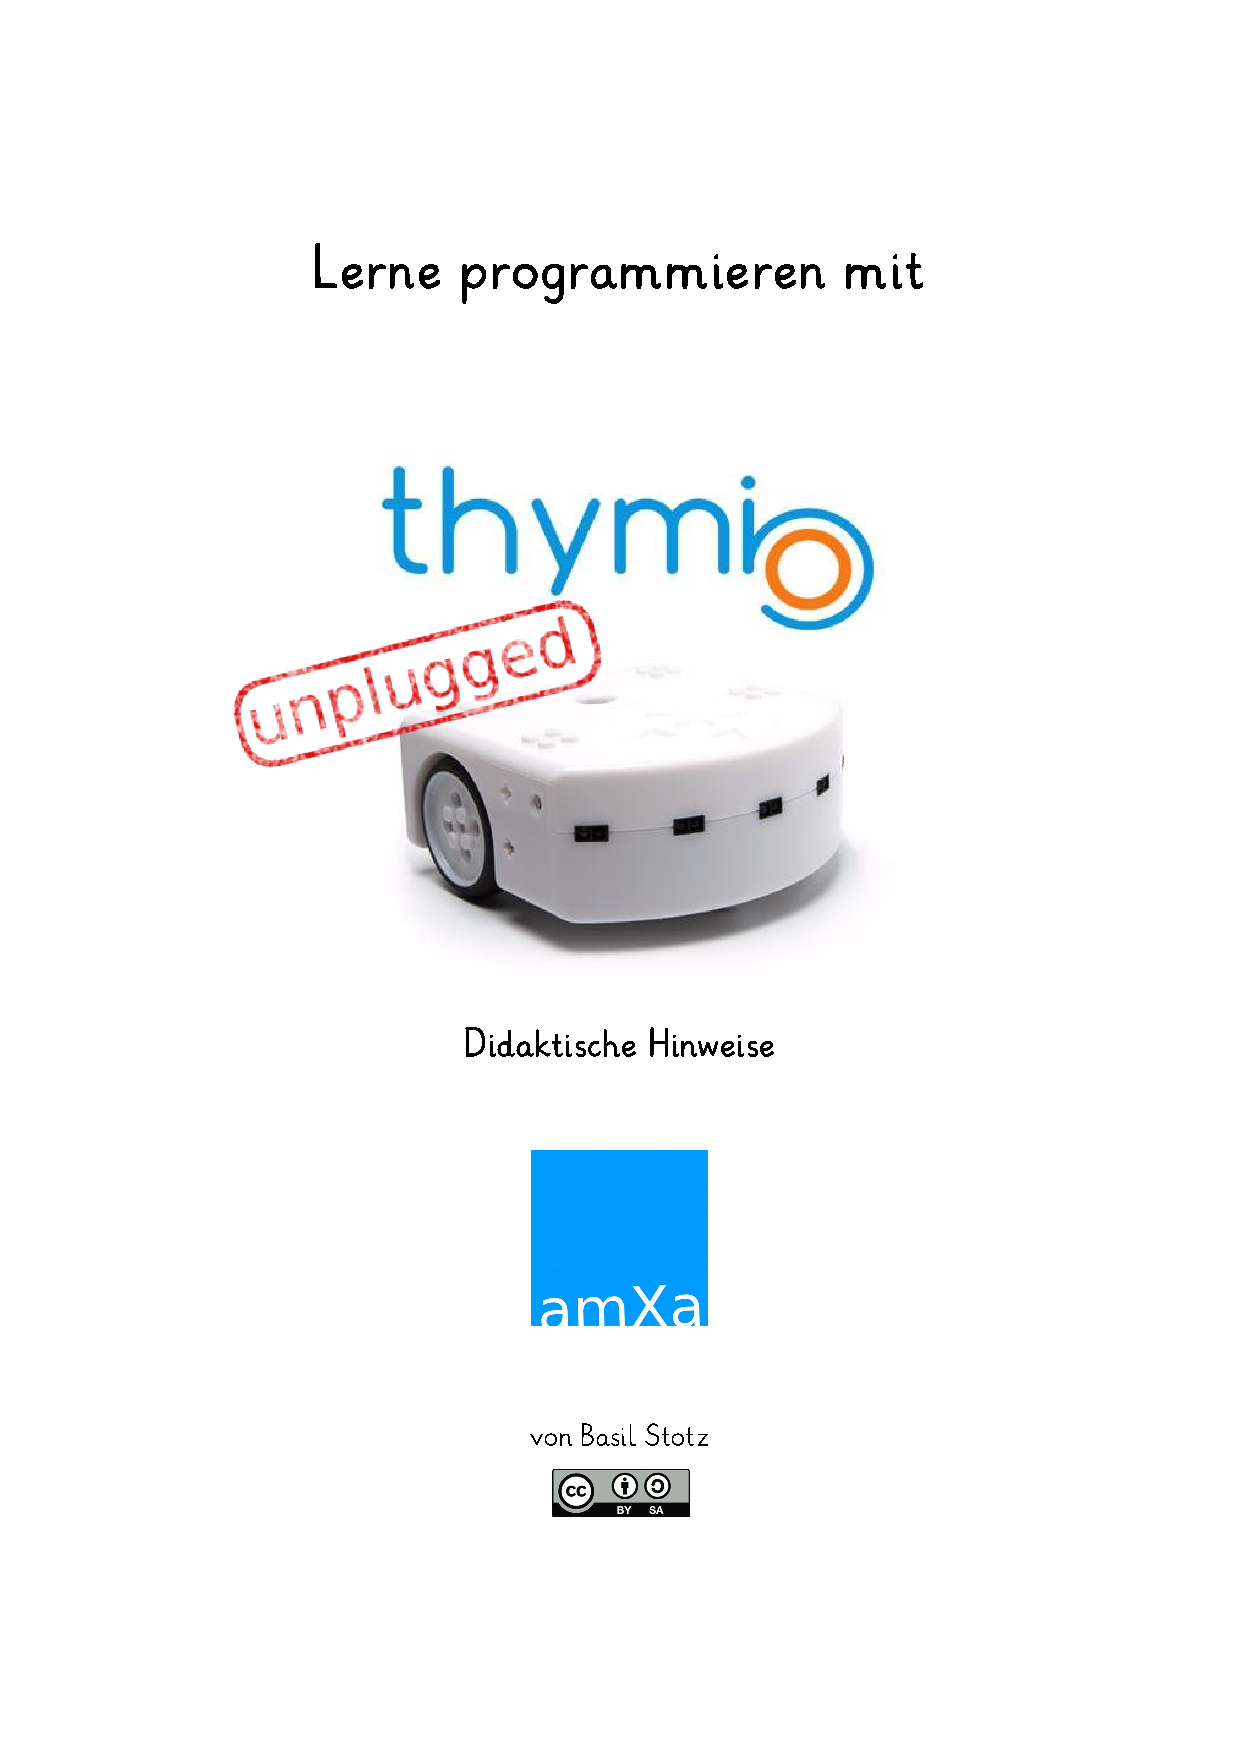
\includepdf{Thymio-HPL-GS-LuL.pdf}

\section*{Einleitung}
Das Ziel dieser Einheit besteht darin, mit dem Thymio erste Schritte der Programmierung zu erleben, nur mit dem Thymio selbst ohne die Hilfe eines Computers oder Tablets zu machen.

Zu diesem Zweck wurde die haptische Programmiersprache {\bf HPL} entwickelt. Die Idee dahinter besteht darin den Roboter in eine bestimmte reale Situation zu bringen und ihm dann eine Anweisung zu seinem Verhalten zu geben. Die Korrektheit des Programms lässt dann sofort in der Praxis überprüfen.

Um das zu erreichen wird die Software des Thymios mit einem speziellen Programm erweitert, welches dies auf einfachste Weise zulässt. 

\subsection*{Voraussetzung}

Die SuS sollen die vorprommierten Verhalten des Thymio selber programmieren. Sie sollen daher die vorprogrammierten Verhalten von Thymio gut kennen, indem sie z.B. die "Einführung in die Welt der Roboter" durchgearbeitet haben. 

\subsection*{Vorbereitung}
Für diese Lerneinheit muss Thymio mit einer SD-Karte mit der Software dieser Einheit versehen werden. Die SD-Karte wird dabei einfach in den {\bf ausgeschalteten} Thymio eingesetzt und gestartet.

Jetzt hat Thymio, zusätzlich zu normalen "farbigen" Verhalten, ein weiteres "farbloses" Ver\-halten. Dieses neue Verhalten wird, wie die Anderen auch, durch berühren der mittleren Taste angewählt\footnote{Einmal angewählt kann dieses Verhalten, im Gegensatz zu den Anderen, aber nur durch einen Neustart des Thymio verlassen werden. Wird die Karte, wieder bei {\bf abgeschaltetem} Thymio, entfernt, dann ist Thymio wieder in seinem original Zustand.}.

\subsection*{Material}

Folgendes Material wird pro SuS benötigt:

\begin{itemize}
\item ein Satz Kopien der benötigten Arbeitsblätter
\item ein Thymio (mit spezieller SD-Karte)
\item eine kleine weisse (Karton-)Schachtel als Hindernis
\item eine A3-Kopie der 8er Fahrbahn (für das Arbeitsblatt "Thymio fährt auf dem Weg")
\item mindestens $1\,m^2$ Platz auf dem Tisch 
\end{itemize}

Es ist auch möglich, dass sich zwei SuS einen Thymio teilen.


\subsection*{Ablauf}

Es gibt eine Basisversion und eine erweiterte Version. In der Basisversion werden nur die vorderen Distanzsensoren verwendet. Dies sind am einfachsten zu programmieren. Die erweiterte Version kann zur Binnendifferenzierung oder für spezielle Kurse genutzt werden.

\begin{center}
\begin{tabular}{|l|c|c|c|p{3cm}|}
\hline
{\bf Arbeitsblatt} &{\bf Sensor} &{\bf Niveau}&{\bf Zeit} &{\bf Bemerkungen}\\\hline
%Die Sinne des Thymio & Alle &erweitert &30 &evtl. ohne AB\\\hline
Thymio ist gehorsam & ----- & basis & 30&evtl. ohne AB\\\hline
Thymio ist freundlich  &Sehen (vorne) & basis&20&\\\hline
Thymio ist ängstlich  &Sehen (vorne) & basis&20 &\\\hline
Thymio ist neugierig &Sehen (vorne)  & basis &20 &\\\hline
Thymio fährt auf dem Weg & Sehen (unten) & erweitert&30&\\\hline
Thymio ist aufmerksam & Hören & erweitert&30&\\\hline
Thymio eckt an & Gleichgewicht & erweitert&30&\\\hline
\end{tabular}
\end{center}



\subsection*{Anleitung zum Programm}

Wenn das neue farblose Verhalten angewählt wurde leuchtet der Roboter in gelb und ist bereit. Durch ein kurzes\footnote{Frage: Wäre lang besser?} Berühren der mittleren Taste wechselt er in den Programmiermodus und wird weiss. 

Jetzt wird der Roboter in die gewünschte Stuation gebracht, indem vorne, rechts oder links ein Hindernis hingestellt wird\footnote{An den roten LEDs bei den horizontalen Distanzsensoren wird die Wahrnehmung der Roboters (vorne, links oder rechts) optisch dargestellt.}. Am besten eignet sich eine kleine, weisse Kartonschachtel dazu.

Im nächsten Schritt wird die zu diesem Verhalten benötigte Handlungsanweisung durch (kurzes) Berühren einer der fünf Tasten festgelegt.

Dies beiden Schritte werden dann für alle relevanten Situationen des Roboters wiederholt.

Die Programmierung wird durch langes Berühren (etwa eine Sekunde) beendet. Das eingegebene Programm wird dann gestartet und der Roboter wird grün.

Mit einer kurzen Berührung der mittleren Taste wechselt der Roboter wieder in den Bereitschaftsmodus.

Mit der Rückwärts-Taste kann das eben programmierte Verhalten neu gestartet werden oder mit einem kurzen\footnote{Frage: Wäre lang besser?}  Click auf der mittleren Taste neu programmiert werden. 

Werden im Bereitschaftsmodus (gelb) die Links- und Rechts-Taste gleichzeitig während etwa 10 Sekunden gedrückt, dann wechselt Thymio den benutzten Sinn. Thymio sagt dann welcher Sinn aktiv ist.

\subsection*{Hinweise zur Durchführung}

Die Fahrtrichtungsangaben sind immer auf den Roboter selbst bezogen. Es ist daher sinnvoll den Roboter immer in gleicherweise, wie in den Bildern dargestellt, nach oben auszurichten.

\subsection*{Eine Speicherkarte herstellen}

Normalerweise sollte die SD-Karte schon vorhanden sein und kannst diesen Abschnitt überspringen.
 
Falls du aber keine SD-Karte hast, wird hier beschrieben, wie du eine solche Karte selber herstellen kannst.

Als SD-Karte kannst du jede handelsübliche microSD-Karte verwenden. Je weniger Kapazität die Karte hat umso besser, es geht aber auch mit 64 GByte Karte.

Neurere SD-Karten sind häufig mit einem eFat-Filesystem formatiert. Die Karte muss aber als vfat-Dateisystem formatiert sein. Falls die Karte mit einem anderen Dateisystem formatiert ist, musst du diese auf vfat umformatieren. Verwende dazu das Programm gparted (Linux), Diskutility (macOS) oder xxxxxx (Windows).

Lade einfach die Datei xxxxxxxxxxx herunter, entpacke sie und kopiere alle Dateien, mit drag‘n‘drop, auf die SD-Karte. Fertig

\newpage
%\section*{Arbeitsblätter}

\section*{Die Sinne des Thymio}

\subsection*{Ziel}

Die SuS (er-)kennen die verschiedenen Sensoren des Thymio und können diese am Roboter lokalisieren. Als Zusatz können auch die Sinne des Menschen besprochen werden.

\subsection*{Beschreibung}

Der Thymio besitzt fünf Sensorgruppen, von denen aber nur vier verwendet werden\footnote{Der haptische Sinn (Fühlen) wird hier nicht benutzt. Diese Tasten werden zur Motorensteuerung verwendet}:

\begin{center}
%\begin{table}[h]
\begin{tabular}[b]{|c|p{5cm}|p{5cm}|}
\hline
\bf Sinn&\bf Beschreibung&\bf Bemerkung\\\hline
%\raisebox{-0.75\height}{\includesvg[width=0.15\textwidth]{event-buttons}}&{\bf Fühlen} &Dieser Sinn wird hier nicht benutzt. Diese Tasten werden hier zur Motorensteurung verwendet\\\hline
\raisebox{-0.75\height}{\includesvg[width=0.15\textwidth]{event-prox}}&{\bf Sehen (Umgebung)}\par Es werden die nur die vorderen 5 Distanzsensoren genutzt.& {\bf Die vorderen Distanzsensoren werden als Vorgabe benutzt.}\\\hline
\raisebox{-0.75\height}{\includesvg[width=0.15\textwidth]{event-ground}}&{\bf Sehen (Boden)}\par & \\\hline
\raisebox{-0.75\height}{\includesvg[width=0.15\textwidth]{event-tap}}&{\bf Gleichgewicht}\par Wird hier zum dedektieren und zählen von Schlägen/Klopfen verwendet. & \\\hline
\raisebox{-0.75\height}{\includesvg[width=0.15\textwidth]{event-clap}}&{\bf Hören}\par Der Hörsinn zum dedektieren und zählen vom Klatschen verwendet.& Der Hörsinn nicht gut verwendet werden, weil die Geräusche der anderen SuS stören.\\\hline
\end{tabular}
%\end{table}
\end{center}

In der Basisversion werden nur die vorderen Distanzsensoren benutzt, daher kann dieses AB auch weggelassen werden. 

%\subsection*{Ablauf}

%\newpage
\section*{Thymio ist gehorsam}

\subsection*{Ziel}

Die AB ist als Vorbereitung zur Programmierung gedacht: Die SuS lernen die Bedeutung der fünf "Bewegungstasten" und die Begriffe 'stopp' 'links', 'rechts', 'vorwärts' und 'rückwärts'.

\subsection*{Beschreibung}

In der HPL-Sprache gibt es fünf mögliche Aktionen, denen jeweils eine Taste zugeordnet ist.

Die Richtungswechsel und die Rückwartsfahrten sollen darauf sensibilisieren, dass Richtungangaben je nach Sichtweise ändern können. Imbesonderen soll gelernt werden, dass die Richtungangaben immer relativ zum Roboter zu verstehen sind.

\subsection*{Ablauf}

Auf dem Tisch wird ein Hindernis aufgestellt und die SuS sollen mit dem lila Verhalten händisch um das Hindernis herum fahren. 

Die AB kann auch mit dem "gewöhnlichen" lila Verhalten gemacht werden, allerdings fehlt dort die Stopp-Taste.

%\newpage
\section*{Thymio ist freundlich}
\subsection*{Ziel}
Das grüne Verhalten des Thymios soll von den SuS mit HPL selber programmiert werden.

%\subsection*{Beschreibung}



\subsection*{Ablauf}

In einem ersten Schritt füllen die SuS das AB aus, indem sie die korrekte Fahranweisung, das heisst die korrekte Taste rot anmalen. Im zweiten Schritt probieren sie ihr Programm aus.

%\newpage
\section*{Thymio ist ängstlich}
\subsection*{Ziel}
Das rote Verhalten des Thymios soll von den SuS mit HPL selber programmiert werden.


%\subsection*{Beschreibung}



\subsection*{Ablauf}
In einem ersten Schritt füllen die SuS das AB aus, indem sie die korrekte Fahranweisung, das heisst die korrekte Taste rot anmalen. Im zweiten Schritt probieren sie ihr Programm aus.


%\newpage
\section*{Thymio ist neugierig}
\subsection*{Ziel}
Das gelbe Verhalten des Thymios soll von den SuS mit HPL selber programmiert werden.
%\subsection*{Beschreibung}
\subsection*{Ablauf}
In einem ersten Schritt füllen die SuS das AB aus, indem sie die korrekte Fahranweisung, das heisst die korrekte Taste rot anmalen. Im zweiten Schritt probieren sie ihr Programm aus.

%\newpage
\section*{Thymio fährt auf einem Weg}
\subsection*{Ziel}
Das hellblaue Verhalten des Thymios soll von den SuS mit HPL selber programmiert werden.
%\subsection*{Beschreibung}
\subsection*{Ablauf}
In einem ersten Schritt füllen die SuS das AB aus, indem sie die korrekte Fahranweisung, das heisst die korrekte Taste rot anmalen. Im zweiten Schritt probieren sie ihr Programm aus.

%\newpage
\section*{Thymio ist aufmerksam}
\subsection*{Ziel}
Das dunkelblaue Verhalten des Thymios soll von den SuS mit HPL selber programmiert werden.
\subsection*{Beschreibgung}
Das extakte Verhalten des dunkelblauen Thymios lässt sich mit HPL nicht nachbilden.   Es können daher frei gewählte Fahrbefehle benutzt werden.
\subsection*{Ablauf}
In einem ersten Schritt füllen die SuS das AB aus, indem sie die korrekte Fahranweisung, das heisst die korrekte Taste rot anmalen. Im zweiten Schritt probieren sie ihr Programm aus.

%\newpage
\section*{Thymio eckt an}
\subsection*{Ziel}
Ein dem dunkelblauen ähnliches Verhalten, aber mit dem Gleichgewichtssinn,  soll von den SuS mit HPL selber programmiert werden.
\subsection*{Beschreibung}
Diese Verhalten benutzt der "gewöhnliche" Thymio nicht. Es können daher frei gewählte Fahrbefehle benutzt werden.
\subsection*{Ablauf}
In einem ersten Schritt füllen die SuS das AB aus, indem sie die korrekte Fahranweisung, das heisst die korrekte Taste rot anmalen. Im zweiten Schritt probieren sie ihr Programm aus.


\end{document}